\documentclass[10.5pt]{article}
\usepackage{amsmath,amssymb,amsthm}
\usepackage{listings}
\usepackage{graphicx}
\usepackage[shortlabels]{enumitem}
\usepackage{tikz}
\usepackage[margin=1in]{geometry}
\usepackage{fancyhdr}
\usepackage{epsfig} %% for loading postscript figures
\usepackage{amsmath}
\usepackage{float}
\usepackage{amssymb}
\usepackage{caption}
\usepackage{subfigure}
\usepackage{graphics}
\usepackage{titlesec}
\usepackage{mathrsfs}
\usepackage{amsfonts}
\usepackage{indentfirst}
\usepackage{fancybox}
\usepackage{tikz}
\usepackage{algorithm}
\usepackage{algorithmic}

\renewcommand{\baselinestretch}{1.2}%Adjust Line Spacing
%\geometry{left=2.0cm,right=2.0cm,top=2.0cm,bottom=2.0cm}% Adjust Margins of the File
\usepackage{tikz-qtree}
\usetikzlibrary{graphs}
\tikzset{every tree node/.style={minimum width=2em,draw,circle},
	blank/.style={draw=none},
	edge from parent/.style=
	{draw,edge from parent path={(\tikzparentnode) -- (\tikzchildnode)}},
	level distance=1.2cm}
\setlength{\parindent}{0pt}
%\setlength{\parskip}{5pt plus 1pt}
\setlength{\headheight}{13.6pt}
\newcommand\question[2]{\vspace{.25in}\hrule\textbf{#1: #2}\vspace{.5em}\hrule\vspace{.10in}}
\renewcommand\part[1]{\vspace{.10in}\textbf{(#1)}}
%\newcommand\algorithm{\vspace{.10in}\textbf{Algorithm: }}
\newcommand\correctness{\vspace{.10in}\textbf{Correctness: }}
\newcommand\runtime{\vspace{.10in}\textbf{Running time: }}
\pagestyle{fancyplain}
% Create horizontal rule command with an argument of height
\newcommand{\horrule}[1]{\rule{\linewidth}{#1}}
% Set the title here
\title{
	\normalfont \normalsize
	\textsc{ShanghaiTech University} \\ [25pt]
	\horrule{0.5pt} \\[0.4cm] % Thin top horizontal rule
	\huge CS101 Algorithms and Data Structures\\ % The assignment title
	\LARGE Fall 2019\\
	\LARGE Homework 8\\
	\horrule{2pt} \\[0.5cm] % Thick bottom horizontal rule
}
% wrong usage of \author, never mind
\author{}
\date{Due date: 23:59, November 17, 2019}

% set the header and footer
\pagestyle{fancy}
\lhead{CS101 Algorithms and Data Structures}
\chead{Homework 8}
\rhead{Due date: 23:59, November 17, 2019}
\cfoot{\thepage}
\renewcommand{\headrulewidth}{0.4pt}
\newtheorem{Q}{Question}
% special settings for the first page
\fancypagestyle{firstpage}
{
	\renewcommand{\headrulewidth}{0pt}
	\fancyhf{}
	\fancyfoot[C]{\thepage}
}

% Add the support for auto numbering
% use \problem{title} or \problem[number]{title} to add a new problem
% also \subproblem is supported, just use it like \subsection
\newcounter{ProblemCounter}
\newcounter{oldvalue}
\newcommand{\problem}[2][-1]{
	\setcounter{oldvalue}{\value{secnumdepth}}
	\setcounter{secnumdepth}{0}
	\ifnum#1>-1
	\setcounter{ProblemCounter}{0}
	\else
	\stepcounter{ProblemCounter}
	\fi
	\section{Problem \arabic{ProblemCounter}: #2}
	\setcounter{secnumdepth}{\value{oldvalue}}
}
\newcommand{\subproblem}[1]{
	\setcounter{oldvalue}{\value{section}}
	\setcounter{section}{\value{ProblemCounter}}
	\subsection{#1}
	\setcounter{section}{\value{oldvalue}}
}

\begin{document}
	\maketitle
	\thispagestyle{firstpage}
	%\newpage
	\vspace{3ex}
	
	\begin{enumerate}
		\item Please write your solutions in English. 
		
		\item Submit your solutions to gradescope.com.  
		
		\item Set your FULL Name to your Chinese name and your STUDENT ID correctly in Account Settings. 
		
		\item If you want to submit a handwritten version, scan it clearly. Camscanner is recommended. 
		
		\item When submitting, match your solutions to the according problem numbers correctly. 
		
		\item No late submission will be accepted.
		
		\item Violations to any of above may result in zero score. 
	\end{enumerate}
	\newpage
	
	%---------------------------------------------------------
\question{1}{(3*2'+4') Dijkstra's Algorithm}
\begin{Q}
	Judge whether the following statement is true or false and explain why. Give a counter-example if it is false.
	\begin{enumerate}[(a)]
		\item Suppose $G$ is strongly connected with integer edge weights, and has shortest paths from some
		vertex $v$ (i.e. a finite weight shortest path exists from $v$ to all nodes). Then shortest paths can be found from every vertex to every other vertex.
		\par\rm\textbf{Solution:}
		\par\textbf{True.} Since $G$ has shortest paths from some vertices $v$, there should be no negative cycle in $G$, otherwise the shortest path is undefined. Since $G$ is a strongly connected graph, there must be a path between any pair of vertices and the above property implies that there must be a shortest path between any pair of vertices.
		\vspace{8pt}
		\item If G is a connected and undirected graph without negative cycles, we can apply Dijkstra's algorithm to find the shortest path.
		\par\textbf{Solution:}
		\par\textbf{True.} Suppose there's no shortest path between any pair of vertices, then those two vertices are either unconnected or there's a negative edge between and both conditions are contradictory to the question. Thus there must be a shortest path. The Dijkstra's algorithm always finds a shortest edge between the visited and unvisited parts so it can find that shortest path.
		\vspace{8pt}
		\item Suppose $G$ is a DAG. We can find the longest path by negating all edge lengths and then run Dijkstra's algorithm from every source node.
		\par\textbf{Solution:}
		\par\textbf{False.} Consider the following two graphs:
		\begin{figure}[htbp]
		\centering
		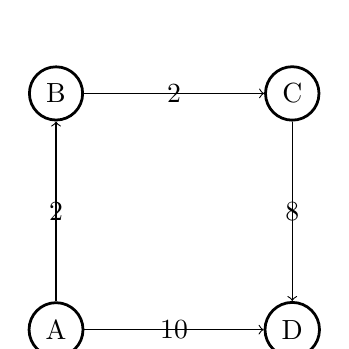
\begin{tikzpicture}
		\centering
		[thick,scale=0.8, every node/.style={scale=1}]
		%		\node[circle] (n0){A};
		\node[circle, draw, line width=1pt] (a) at (-6,0){A};
		\node[circle, draw, line width=1pt] (b) at (-6,3){B};
		\node[circle, draw, line width=1pt] (c) at (-3,3){C};
		\node[circle, draw, line width=1pt] (d) at (-3,0){D};
		\draw[->] (a) to node{2} (b);
		\draw[->] (a) to node{10} (d);
		\draw[->] (b) to node{2} (c);
		\draw[->] (c) to node{8} (d);
		\end{tikzpicture}
		\hspace{0.8in}
		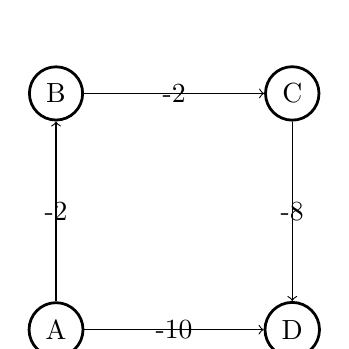
\begin{tikzpicture}
		\centering
		[thick,scale=0.8, every node/.style={scale=1}]
		%		\node[circle] (n0){A};
		\node[circle, draw, line width=1pt] (a) at (-6,0){A};
		\node[circle, draw, line width=1pt] (b) at (-6,3){B};
		\node[circle, draw, line width=1pt] (c) at (-3,3){C};
		\node[circle, draw, line width=1pt] (d) at (-3,0){D};
		\draw[->] (a) to node{-2} (b);
		\draw[->] (a) to node{-10} (d);
		\draw[->] (b) to node{-2} (c);
		\draw[->] (c) to node{-8} (d);
		\end{tikzpicture}
	\end{figure}
	\par By negating all edge lengths of the left graph, we obtain the right graph.\\
	By running the Dijkstra's algorithm on the right graph, the longest path from vertex $A$ to vertex $D$ is $A - D$, however, the actual longest path from $A$ to $D$ is $A - B - C - D$, which can be obtained form the left graph.
		\pagebreak
		
	\end{enumerate}
\end{Q}

\begin{Q}
	Given a weighted graph below, please run Dijkstra's algorithm using vertex $A$ as the source. Write down the vertices in the order which they are marked and the updated distances at each step.
	
	\begin{figure}[htbp]
		\centering
		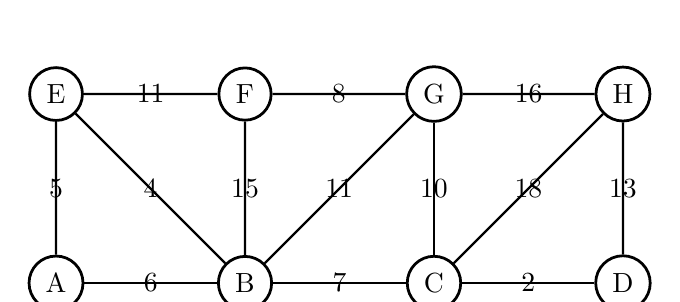
\begin{tikzpicture}
		[thick,scale=0.8, every node/.style={scale=1}]
		%		\node[circle] (n0){A};
		\node[circle, draw, line width=1pt] (a) at (-4.5,0){A};
		\node[circle, draw, line width=1pt] (b) at (-1.5,0){B};
		\node[circle, draw, line width=1pt] (c) at (1.5,0){C};
		\node[circle, draw, line width=1pt] (d) at (4.5,0){D};
		\node[circle, draw, line width=1pt] (e) at (-4.5,3){E};
		\node[circle, draw, line width=1pt] (f) at (-1.5,3){F};
		\node[circle, draw, line width=1pt] (g) at (1.5,3){G};
		\node[circle, draw, line width=1pt] (h) at (4.5,3){H};
		\draw[-] (a) to node{6} (b);
		\draw[-] (a) to node{5} (e);
		\draw[-] (b) to node{7} (c);
		\draw[-] (b) to node{4} (e);
		\draw[-] (b) to node{15} (f);
		\draw[-] (b) to node{11} (g);
		\draw[-] (c) to node{2} (d);
		\draw[-] (c) to node{10} (g);
		\draw[-] (c) to node{18} (h);
		\draw[-] (d) to node{13} (h);
		\draw[-] (e) to node{11} (f);
		\draw[-] (f) to node{8} (g);
		\draw[-] (g) to node{16} (h);
		\end{tikzpicture}
	\end{figure}
	\vspace{10pt}
	\rm\textbf{Solution}:
	\vspace{-15pt}
	\begin{table}[htbp]
		\begin{center}  
			\begin{tabular}{|c|c| p{3cm}|}  
				\hline  
				step & vertex\\ \hline  
				1 &A   \\ \hline    
				2 &E   \\ \hline    
				3 &B   \\ \hline    
				4 &C   \\ \hline    
				5 &D   \\ \hline   
				6 &F   \\ \hline    
				7 &G   \\ \hline   
				8 &H   \\  
				\hline  
			\end{tabular}  
		\end{center}  
	\end{table}
	\vspace{-25pt}
	\begin{table}[htbp]
		\begin{center}  
			\begin{tabular}{|c|c|c|c|c|c|c|c|c| p{3cm}|}  
				\hline  
				step & dist[A] & dist[B] & dist[C] & dist[D] & dist[E] & dist[F] & dist[G] & dist[H]\\ \hline  
				1 &0   &6   &$\infty$   & $\infty$   &5   & $\infty$    & $\infty$   & $\infty$  \\ \hline    
				2 &0   &6   & $\infty$   & $\infty$   &5   &16   & $\infty$   & $\infty$  \\ \hline    
				3 &0   &6   &13   & $\infty$   &5   &16   &17   & $\infty$  \\ \hline    
				4 &0   &6   &13   &15   &5   &16   &17   &31  \\ \hline    
				5 &0   &6   &13   &15   &5   &16   &17   &28  \\ \hline   
				6 &0   &6   &13   &15   &5   &16   &17   &28  \\ \hline    
				7 &0   &6   &13   &15   &5   &16   &17   &28  \\ \hline   
				8 &0   &6   &13   &15   &5   &16   &17   &28  \\  
				\hline  
			\end{tabular}  
		\end{center}  
	\end{table}
\end{Q}
\pagebreak
%---------------------------------------------------------
\question{2}{(2'+3') Floyd-Warshall Algorithm}	
\begin{Q}
	Let $G=(V,E)$ be a connected, undirected graph with edge weights $w:E\rightarrow \mathbb{Z}$. Which of the following statements are True about the Floyd-Warshall algorithm applied to $G$?
	\begin{enumerate}[(A)]
		\item Since G is undirected, we cannot apply Floyd-Warshall algorithm.
		\item Since G is undirected, Floyd-Warshall will be asymptotically faster than on directed graphs.
		\item Since G is undirected, Floyd-Warshall will be unable to detect negative-weight cycles.
		\item None of the above.
	\end{enumerate}
\end{Q}
\par\textbf{Solution: C}
\pagebreak

\begin{Q}
	Consider the following implementation of the Floyd-Warshall algorithm. Assume $w_{ij}=\infty$ where there is no edge between vertex $i$ and vertex $j$, and assume $w_{ii}=0$ for every vertex $i$.
	\begin{algorithm}
		\caption{Floyd-Warshall}
		\label{alg:Floyd-Warshall}
		\begin{algorithmic}
			\FOR{$i=1$ to $n$}
			\FOR{$j=1$ to $n$}
			\STATE $A[i,j,0]=w_{ij}$
			\STATE $P[i, j] = -1$
			\ENDFOR
			\ENDFOR
			\FOR{$k=1$ to $n$}
			\FOR{$i=1$ to $n$}
			\FOR{$j=1$ to $n$}
			\STATE $A[i, j, k] = A[i, j, k - 1]$
			\IF{$A[i, j, k] > A[i, k, k - 1] + A[k, j, k - 1]$}
			\STATE $A[i, j, k] = A[i, k, k - 1] + A[k, j, k - 1]$
			\STATE $P[i, j] = k$
			\ENDIF
			\ENDFOR
			\ENDFOR
			\ENDFOR
		\end{algorithmic}
	\end{algorithm}
	
	Assume matrix $P$, the output of the above algorithm is given. Consider the following matrix for graph $G$ with $7$ vertices. What is the shortest path from vertex $5$ to vertex $7$ in graph $G$?
	
	\begin{table}[htbp]
		\begin{center}  
			\begin{tabular}{|c|c|c|c|c|c|c|c|c| p{3cm}|}  
				\hline  
				P & 1 & 2 & 3 & 4 & 5 & 6 & 7\\ \hline  
				1 & -1 & 5 & 4 & -1 & 4 & 4 & -1\\ \hline    
				2 & 5 & -1 & 5 & 5 & -1 & 5 & -1\\ \hline    
				3 & 4 & 5 & -1 & -1 & -1 & -1 & 6\\ \hline    
				4 & -1 & 5 & -1 & -1 & 3 & 3 & 1\\ \hline    
				5 & 4 & -1 & -1 & 3 & -1 & 3 & 6\\ \hline   
				6 & 4 & 5 & -1 & 3 & 3 & -1 & -1\\ \hline    
				7 & -1 & -1 & 6 & 1 & 6 & -1 & -1\\ 
				\hline  
			\end{tabular}  
		\end{center}  
	\end{table}
\end{Q}
\par\textbf{Solution:}
\par\textbf{The shortest path is }\boldmath$5 - 3 - 6 - 7.$\unboldmath \: 	Since $P[5,7] == 6$, the shortest path must pass vertex 6; Since $P[6,7] == -1$, which means edge $6 - 7$ is the shortest path from vertex 6 to vertex 7; Since the $P[5,6] == 3$, the path from vertex 5 to vertex 6 must pass vertex 3; Since $P[5,3] == -1$, the edge $5 - 3$ is part of the path; Since $P[3,6] == -1$, the edge $3 - 6$ is part of the path; Thus the next vertex of vertex 5 is vertex 3, the next vertex of vertex 3 is vertex 6, the next vertex of vertex 6 is vertex 7; Therefore, the shortest path from vertex 5 to vertex 7 is $5 - 3 - 6 - 7$.
\pagebreak
%---------------------------------------------------------	
\question{3}{(3'+3'+4') Shortest Path}
\begin{Q}
	Consider a weighted undirected graph with positive edge weights and let $(u,v)$ be an edge in the graph. It is known that the shortest path from the source vertex $s$ to $u$ has weight $53$ and the shortest path from $s$ to $v$ has weight $65$. Which is the range of the weight the edge $(u,v)$?
\end{Q}
\par\textbf{Solution:}
\par\boldmath$weight(u,v) >= 12.$\unboldmath\: Motivated by triangular, we can obtain $dist(s,v) + weight(v,u) >= dist(s,u)$, thus $weight(u,v) >= dist(s,u) - dist(s,v) = 12$.\\
Therefore, $weight(u,v) >= 12$.
\vspace{120pt}
\begin{Q}
	Consider the weighted undirected graph with $4$ vertices, where the weight of edge $\{i,j\}$ is given by the entry $W_{i,j}$ in the matrix $W$
	
	$$W=\begin{bmatrix} 0 & 2 & 8 & 6\\ 2 & 0 & 5 & 8\\ 8 & 5 & 0 & x\\ 6 & 8 & x & 0 \end{bmatrix}$$
	
	We want to find the largest possible integer value of $x$, for which at least one shortest path between some pairs of vertices will definitely contain the edge with weight $x$. What is this largest possible integer value of such $x$? Explain your reason briefly. \textbf{When breaking tie, the path may be random.}
\end{Q}
\par\textbf{Solution:}
\par \boldmath$max\{x\} = 12.$\unboldmath\: Since the edge of weight $x$ must be contained in at least one shortest path between some pair of vertices, i.e. the edge between the third and fourth vertices is part of the shortest path, then consider the marginal situation, when the weight of that edge is equal to the weight of the "shortest path" from the third vertex to the fourth vertex through all the other vertices but doesn't contain $x$, then the shortest path from third vertex to the fourth vertex will not contain $x$ because $x$ is too large and will be ignored, so the maximum of $x$ is that weight minus 1. The "shortest path" mentioned is: 3rd - 2nd - 1st - 4th.\\
Therefore, $max\{x\} == 5 + 2 + 6 - 1= 12$. 
\vspace{120pt}
\pagebreak
\begin{Q}
	Suppose $G = (V, E)$ is a weighted graph and $T$ is its shortest-path tree from source $s$. If we increase all weights in $G$ by the same amount, i.e., $\forall e \in E$, $w'_e = w_e + c$. Is $T$ still the shortest-path tree (from source $s$) of the new graph? If yes, prove the statement. Otherwise, give a counter example.
\end{Q}
\par\textbf{Solution:}
\par\textbf{No.} Consider the following two graphs:
\begin{figure}[htbp]
		\centering
		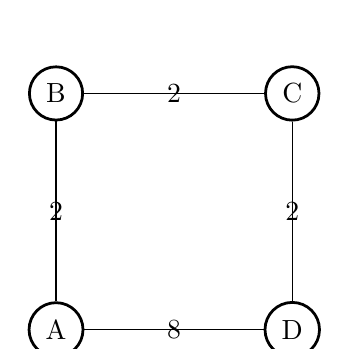
\begin{tikzpicture}
		\centering
		[thick,scale=0.8, every node/.style={scale=1}]
		%		\node[circle] (n0){A};
		\node[circle, draw, line width=1pt] (a) at (-6,0){A};
		\node[circle, draw, line width=1pt] (b) at (-6,3){B};
		\node[circle, draw, line width=1pt] (c) at (-3,3){C};
		\node[circle, draw, line width=1pt] (d) at (-3,0){D};
		\draw[-] (a) to node{2} (b);
		\draw[-] (a) to node{8} (d);
		\draw[-] (b) to node{2} (c);
		\draw[-] (c) to node{2} (d);
		\end{tikzpicture}
		\hspace{0.8in}
		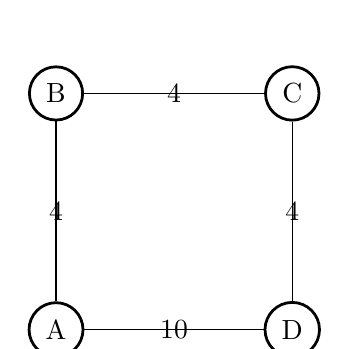
\begin{tikzpicture}
		\centering
		[thick,scale=0.8, every node/.style={scale=1}]
		%		\node[circle] (n0){A};
		\node[circle, draw, line width=1pt] (a) at (-6,0){A};
		\node[circle, draw, line width=1pt] (b) at (-6,3){B};
		\node[circle, draw, line width=1pt] (c) at (-3,3){C};
		\node[circle, draw, line width=1pt] (d) at (-3,0){D};
		\draw[-] (a) to node{4} (b);
		\draw[-] (a) to node{10} (d);
		\draw[-] (b) to node{4} (c);
		\draw[-] (c) to node{4} (d);
		\end{tikzpicture}
		
\end{figure}
\par The left graph is the original $G$ and the path from vertex A to vertex D in its shortest-path tree $T$ is $A - B - C - D$; The right graph is obtained from increase all weights in the left graph by 2, the the path from vertex A to vertex D in its shortest-path tree $T'$ is $A - D$. Therefore $T$ is not the shortest-path tree of the new graph.
	
\end{document}